%% Submissions for peer-review must enable line-numbering
%% using the lineno option in the \documentclass command.
%%
%% Preprints and camera-ready submissions do not need
%% line numbers, and should have this option removed.
%%
%% Please note that the line numbering option requires
%% version 1.1 or newer of the wlpeerj.cls file.

\documentclass[fleqn,10pt,lineno,numbers]{wlpeerj} % for journal submissions
% \documentclass[fleqn,10pt]{wlpeerj} % for preprint submissions

%\usepackage[numbers]{natbib}

\usepackage{lmodern}
\usepackage[T1]{fontenc}
\usepackage[utf8]{inputenc}
\usepackage[scaled=0.8]{DejaVuSansMono}

\usepackage{hyperref}
\usepackage{graphicx}
\usepackage[all]{xy}
\usepackage{amsmath}
\usepackage{caption}
\graphicspath{ {images/} }

% Makes quote characters in monospace font not be curly
\usepackage{upquote}

\usepackage{amsmath}
\usepackage{url}
\usepackage{hyperref}

% this is required for all the \url{} commands in the bib file
%\usepackage{hyperref}

% for nice units
\usepackage{siunitx}

% for images: png, pdf, etc
\usepackage{graphicx}

% for nice table formatting, i.e., /toprule, /midrule, etc
\usepackage{booktabs}

% to allow for \verb++ declarations in captions.
\usepackage{cprotect}

% to allow usage of \mathbb symbols
\usepackage{amssymb}

\usepackage{longtable}

\usepackage{listings}


\begin{document}

\flushbottom
\thispagestyle{empty}%
\vskip-36pt%
{\raggedright\sffamily\bfseries\fontsize{20}{25}\selectfont SymPy: Symbolic Computing in Python\par}%
\vskip10pt
{\raggedright\sffamily\fontsize{12}{16}\selectfont  Supplementary material\par}
\vskip25pt%

The supplementary material take a deeper look at certain topics in SymPy for
which there was not enough room to discuss in the paper.
Section~\ref{suppsec:Gruntz} discusses the Gruntz algorithm, used to
calculate limits in the SymPy.  Sections~\ref{suppsec:Series}--\ref{suppsec:Ten}
discuss in depth some selected submodules.  Section~\ref{suppsec:numsimpl}
discusses numerical simplification.  Section~\ref{suppsec:examples} provides
additional examples for topics, discussed in the main paper.  In section
\ref{sympy-gamma} the SymPy Gamma
and the SymPy Live projects are introduced.  Finally, section~\ref{suppsec:comp-mma}
has a
brief comparison of SymPy with Wolfram Mathematica.

As in the paper, all examples in the supplement assume that the following
has been run:
\begin{verbatim}
>>> from sympy import *
>>> x, y, z = symbols('x y z')
\end{verbatim}


\section{Limits: The Gruntz Algorithm}
\label{suppsec:Gruntz}
SymPy calculates limits using the Gruntz algorithm, as described in%
~\cite{Gruntz1996limits}. The basic idea is as follows: any limit can be
converted to a limit $\lim\limits_{x\to\infty} f(x)$ by substitutions like
$x\to{1\over x}$. Then the most varying subexpression $\omega$ (that converges
to zero as $x\to\infty$ the fastest from all subexpressions) is identified in
$f(x)$, and $f(x)$ is expanded into a series with respect to $\omega$. Any
positive powers of $\omega$ converge to zero. If there are negative powers of
$\omega$, then the limit is infinite. The constant term (independent of
$\omega$, but could depend on $x$) then determines the limit (one might need to
recursively apply the Gruntz algorithm on this term to determine the limit).

To determine the most varying subexpression, the comparability classes must
first be defined, by calculating $L$:
\begin{equation}
L\equiv \lim_{x\to\infty} {\log |f(x)| \over \log |g(x)|}
\end{equation}
The relations $<$, $>$, and $\sim$ are defined as follows: $f>g$ when
$L=\pm\infty$ (it is said that $f$ is more rapidly varying than $g$, i.e., $f$
goes to $\infty$ or $0$ faster than $g$), $f<g$ when $L=0$ ($f$ is less
rapidly varying than $g$) and $f\sim g$ when $L\neq 0,\pm\infty$ (both $f$ and
$g$ are bounded from above and below by suitable integral powers of the
other). Note that if $f > g$, then $f > g^n$ for any $n$. Here
are some examples of comparability classes:
$$2 < x < e^x < e^{x^2} < e^{e^x}$$
$$2\sim 3\sim -5$$
$$x\sim x^2\sim x^3\sim {1\over x}\sim x^m\sim -x$$
$$e^x\sim e^{-x}\sim e^{2x}\sim e^{x+e^{-x}}$$
$$f(x)\sim{1\over f(x)}$$

The Gruntz algorithm is now illustrated on the following example:
\begin{equation}
    \label{gruntz_example_fn}
f(x) = e^{x+2e^{-x}} - e^x + {1\over x} \,.
\end{equation}
The goal is to calculate $\lim\limits_{x\to\infty} f(x)$.
First, the set of most rapidly varying subexpressions is determined---the so
called \textit{mrv set}. For~\eqref{gruntz_example_fn}, the mrv set
$\{e^x, e^{-x}, e^{x+2e^{-x}}\}$ is obtained. These are all subexpressions of%
~\eqref{gruntz_example_fn} and they all belong to the same comparability class.
This calculation can be done using SymPy as follows:

% dict_keys output order varies
% no-doctest
\begin{verbatim}
>>> from sympy.series.gruntz import mrv
>>> mrv(exp(x+2*exp(-x))-exp(x) + 1/x, x)[0].keys()
dict_keys([exp(x + 2*exp(-x)), exp(x), exp(-x)])
\end{verbatim}

Next, any item $\omega$ is taken from mrv that converges to zero for
$x\to\infty$. The item $\omega=e^{-x}$ is obtained. If such a term is not
present in the mrv set (i.e., all terms converge to infinity instead of zero),
the relation $f(x)\sim {1\over f(x)}$ can be used.

Next step is to rewrite the mrv in terms of $\omega$: $\{{1\over\omega},
\omega, {1\over\omega}e^{2\omega}\}$. Then the original subexpressions are
substituted back into $f(x)$ and expanded with respect to $\omega$:
\begin{equation}
    \label{gruntz_example_fn2}
f(x) = {1\over x}-{1\over\omega}+{1\over\omega}e^{2\omega}
     = 2+{1\over x} + 2\omega + O(\omega^2)
\end{equation}

Since $\omega$ is from the mrv set, then in the limit $x\to\infty$ it is
$\omega\to0$ and so $2\omega + O(\omega^2) \to 0$ in~\eqref{gruntz_example_fn2}:
\begin{equation}
f(x) = {1\over x}-{1\over\omega}+{1\over\omega}e^{2\omega}
    = 2+{1\over x} + 2\omega + O(\omega^2)
    \to 2 + {1\over x}
\end{equation}

Since the result ($2+{1\over x}$) still depends on $x$, the above procedure is
iterated on the result until just a number (independent of $x$) is obtained,
which is the final limit. In the above case the limit is $2$, as can be
verified by SymPy:

\begin{verbatim}
>>> limit(exp(x+2*exp(-x))-exp(x) + 1/x, x, oo)
2
\end{verbatim}

In general, when $f(x)$ is expanded in terms of $\omega$, it is obtained:
\begin{equation}
f(x) = \underbrace{O\left({1\over \omega^3}\right)}_\infty
    + \underbrace{C_{-2}(x)\over \omega^2}_\infty
    + \underbrace{C_{-1}(x)\over \omega}_\infty
    + {C_{0}(x)}
    + \underbrace{C_{1}(x)\omega}_0
    + \underbrace{O(\omega^2)}_0
\end{equation}
The positive powers of $\omega$ are zero. If there are any negative powers of
$\omega$, then the result of the limit is infinity, otherwise the limit is
equal to $\lim\limits_{x\to\infty} C_0(x)$. The expression $C_0(x)$ is simpler
than $f(x)$ and so the algorithm always converges. A proof of this, as well as
further details are given in Gruntz's PhD thesis~\cite{Gruntz1996limits}.


% Series module (Formal Power Series, Fourier Series)
\section{Series}
\label{suppsec:Series}
% Series expansion (Differentiate between the two approaches being used)
\subsubsection{Series Expansion}

SymPy is able to calculate the symbolic series expansion of an arbitrary series
or expression involving elementary and special functions and multiple
variables. For this it has two different implementations: the \texttt{series}
method and Ring Series.

The first approach stores a series as an instance of the \texttt{Expr} class.
Each function has its specific implementation of its expansion which is able to
evaluate the Puiseux series expansion about a specified point. For example,
consider a Taylor expansion about 0:

\begin{verbatim}
>>> from sympy import symbols, series
>>> x, y = symbols('x, y')
>>> series(sin(x+y) + cos(x*y), x, 0, 2)
1 + sin(y) + x*cos(y) + O(x**2)
\end{verbatim}

The newer and much faster\cite{sympyRingSeries} approach called Ring Series makes use of the
observation that a truncated Taylor series is in fact a polynomial.
Ring Series uses the efficient representation and operations of sparse
polynomials. The choice of sparse polynomials is deliberate, as it performs
well in a wider range of cases than a dense representation. Ring Series gives
the user the freedom to choose the type of coefficients he wants to have in
his series, allowing the use of faster operations on certain types.

For this, several low level methods for expansion of trigonometric, hyperbolic,
and other elementary functions like inverse of a series, calculating $n$th
root, etc, are implemented using variants of the Newton Method~\cite{zimmerman}.
All these support Puiseux series expansion. The following example demonstrates
the use of an elementary function that calculates the Taylor expansion of the
sine of a series.

\begin{verbatim}
>>> from sympy import ring
>>> from sympy.polys.ring_series import rs_sin
>>> R, t = ring('t', QQ)
>>> rs_sin(t**2 + t, t, 5)
-1/2*t**4 - 1/6*t**3 + t**2 + t
\end{verbatim}

The function \texttt{sympy.polys.rs\_series} makes use of these elementary
functions to expand an arbitrary SymPy expression. It does so by following a
recursive strategy of expanding the lower most functions first and then
composing them recursively to calculate the desired expansion. Currently, it
only supports expansion about 0 and is under active development. Ring Series
is several times faster than the default implementation with the speed
difference increasing with the size of the series. The
\texttt{sympy.polys.rs\_series} takes as input any SymPy expression and hence
there is no need to explicitly create a polynomial \texttt{ring}. An example
demonstrating its use:

% rs_series bug, output sometimes has a factored out
% no-doctest
\begin{verbatim}
>>> from sympy.polys.ring_series import rs_series
>>> from sympy.abc import a, b
>>> from sympy import sin, cos
>>> rs_series(sin(a + b), a, 4)
-1/2*(sin(b))*a**2 + (sin(b)) - 1/6*a**3*(cos(b)) + a*(cos(b))
\end{verbatim}

\subsubsection{Formal Power Series}

SymPy can be used for computing the Formal Power Series of a function.
The implementation is based on the algorithm described in the paper on
Formal Power Series~\cite{Gruntz93formalpower}.  The advantage of this approach is
that an explicit formula for the coefficients of the series expansion is generated
rather than just computing a few terms.

The following example shows how to use \texttt{fps}:

\begin{verbatim}
>>> f = fps(sin(x), x, x0=0)
>>> f.truncate(6)
x - x**3/6 + x**5/120 + O(x**6)
>>> f[15]
-x**15/1307674368000
\end{verbatim}

\subsubsection{Fourier Series}

SymPy provides functionality to compute Fourier series of a function using the
\texttt{fourier\_series} function. Under the hood, this function computes $a_0$,
$a_n$, and $b_n$ coefficients using standard integration formulas.

Here's an example on how to compute Fourier series in SymPy:

\begin{verbatim}
>>> L = symbols('L')
>>> expr = 2 * (Heaviside(x/L) - Heaviside(x/L - 1)) - 1
>>> f = fourier_series(expr, (x, 0, 2*L))
>>> f.truncate(3)
4*sin(pi*x/L)/pi + 4*sin(3*pi*x/L)/(3*pi) + 4*sin(5*pi*x/L)/(5*pi)
\end{verbatim}


% Logic module
\section{Logic}
\label{suppsec:Logic}

SymPy supports construction and manipulation of boolean expressions
through the \texttt{sympy.logic} module. SymPy symbols can be used as
propositional variables and also be substituted as \texttt{True}
or \texttt{False}. A good number of manipulation features for boolean
expressions have been implemented in the \texttt{sympy.logic} module.

\subsubsection{Constructing boolean expressions}

A boolean variable can be declared as a SymPy \verb|Symbol|. Python operators
\texttt{\&}, \texttt{\textbar{}} and \texttt{\textasciitilde{}} are overridden
when using SymPy objects
to use the SymPy functionality for logical \texttt{And}, \texttt{Or}, and
\texttt{Not}.  Other logic functions are also integrated into SymPy,
including \texttt{Xor} and \texttt{Implies}, which are constructed with
\texttt{\^{}} and \texttt{\textgreater{}\textgreater{}}, respectively.  The above
are just a shorthand, expressions can also be constructed by directly creating
the relevant objects: \verb|And()|, \verb|Or()|, \verb|Not()|, \verb|Xor()|,
\verb|Nand()|, \verb|Nor()|, etc.

\begin{verbatim}
>>> from sympy import *
>>> x, y, z = symbols('x y z')
>>> e = (x & y) | z
>>> e.subs({x: True, y: True, z: False})
True
\end{verbatim}

\subsubsection{CNF and DNF}

Any boolean expression can be converted to conjunctive normal form, disjunctive
normal form, and negation normal form. The API also exposes methods to check if
a boolean expression is in any of the above mentioned forms.

\begin{verbatim}
>>> from sympy.logic.boolalg import is_dnf, is_cnf
>>> x, y, z = symbols('x y z')
>>> to_cnf((x & y) | z)
And(Or(x, z), Or(y, z))
>>> to_dnf(x & (y | z))
Or(And(x, y), And(x, z))
>>> is_cnf((x | y) & z)
True
>>> is_dnf((x & y) | z)
True
\end{verbatim}

\subsubsection{Simplification and Equivalence}

The module supports simplification of given boolean expression by making
deductions from the expression. Equivalence of two logical expressions can also
be checked. In the case of equivalence, it is possible to return the mapping of
variables in two expressions so as to represent the same logical behavior.

\begin{verbatim}
>>> from sympy import *
>>> a, b, c, x, y, z = symbols('a b c x y z')
>>> e = a & (~a | ~b) & (a | c)
>>> simplify(e)
And(Not(b), a)
>>> e1 = a & (b | c)
>>> e2 = (x & y) | (x & z)
>>> bool_map(e1, e2)
(And(Or(b, c), a), {a: x, b: y, c: z})
\end{verbatim}

\subsubsection{SAT solving}

The module also supports satisfiability (SAT) checking of a given boolean
expression. If satisfiable, it is possible to return a model for which the
expression is satisfiable. The API also supports returning all possible models.
The SAT solver has a clause learning DPLL algorithm implemented with a watch
literal scheme and VSIDS heuristic\cite{moskewicz2008method}.

\begin{verbatim}
>>> from sympy import *
>>> a, b, c = symbols('a b c')
>>> satisfiable(a & (~a | b) & (~b | c) & ~c)
False
>>> satisfiable(a & (~a | b) & (~b | c) & c)
{a: True, b: True, c: True}
\end{verbatim}


\section{Diophantine Equations}
\label{suppsec:Dioph}
Diophantine equations play a central and an important role in number theory.
A Diophantine equation has the form, $f(x_1, x_2, \ldots x_n) = 0$
where $n \geq 2$ and $x_1, x_2, \ldots x_n$ are integer variables. If we can find
$n$ integers $a_1, a_2, \ldots a_n$ such that $x_1 = a_1, x_2 = a_2, \ldots x_n = a_n$
satisfies the above equation, we say that the equation is solvable.

Currently, following five types of Diophantine equations can be solved using
SymPy's Diophantine module.

\begin{itemize}
    \item Linear Diophantine equations: $a_1x_1 + a_2x_2 + \cdots + a_{n}x_{n} = b$
    \item General binary quadratic equation: $ax^2 + bxy + cy^2 + dx + ey + f = 0$
    \item Homogeneous ternary quadratic equation: $ax^2 + by^2 + cz^2 + dxy + eyz + fzx = 0$
    \item Extended Pythagorean equation: $a_{1}x_{1}^2 + a_{2}x_{2}^2 + \cdots + a_{n}x_{n}^2 = a_{n+1}x_{n+1}^2$
    \item General sum of squares: $x_{1}^2 + x_{2}^2 + \cdots + x_{n}^2 = k$
\end{itemize}

When an equation is fed into Diophantine module, it factors the equation (if
possible) and solves each factor separately. Then all the results are combined to
create the final solution set. Following examples illustrate some of the basic
functionalities of the Diophantine module.

\begin{minted}{pycon}
>>> from sympy import symbols
>>> x, y, z = symbols("x, y, z", integer=True)

>>> diophantine(2*x + 3*y - 5)
set([(3*t_0 - 5, -2*t_0 + 5)])

>>> diophantine(2*x + 4*y - 3)
set()

>>> diophantine(x**2 - 4*x*y + 8*y**2 - 3*x + 7*y - 5)
set([(2, 1), (5, 1)])

>>> diophantine(x**2 - 4*x*y + 4*y**2 - 3*x + 7*y - 5)
set([(-2*t**2 - 7*t + 10, -t**2 - 3*t + 5)])

>>> diophantine(3*x**2 + 4*y**2 - 5*z**2 + 4*x*y - 7*y*z + 7*z*x)
set([(-16*p**2 + 28*p*q + 20*q**2, 3*p**2 + 38*p*q - 25*q**2, 4*p**2 - 24*p*q + 68*q**2)])

>>> from sympy.abc import a, b, c, d, e, f
>>> diophantine(9*a**2 + 16*b**2 + c**2 + 49*d**2 + 4*e**2 - 25*f**2)
set([(70*t1**2 + 70*t2**2 + 70*t3**2 + 70*t4**2 - 70*t5**2, 105*t1*t5, 420*t2*t5, 60*t3*t5, 210*t4*t5, 42*t1**2 + 42*t2**2 + 42*t3**2 + 42*t4**2 + 42*t5**2)])

>>> diophantine(a**2 + b**2 + c**2 + d**2 + e**2 + f**2 - 112)
set([(8, 4, 4, 4, 0, 0)])
\end{minted}


% Sets
\section{Sets}
\label{suppsec:Sets}
%% Sets

SymPy supports representation of a wide variety of set, this is achieved by
first defining abstract representation for a smaller number of atomic set
classes and then combining and transforming them using various set operations.

Each of the set class inherits from the base Set class and defines
rules to check membership of a SymPy object, to calculate union, intersection,
set different. In cases we are not able to evaluate these
operations to atomic set classes they are represented as abstract unevaluated
objects.


\begin{itemize}

    % Description of Empty Set sounds too obvious, not sure if we need to keep
    % it.
    \item \textbf{Empty Set}: Nothing is a member of Empty Set. Union with
another set returns the other set and intersection leads to an Empty Set.

    \item \textbf{Universal Set}: Everything is a member of Universal Set.
Union of Universal Set with any set gives Universal Set and intersection leads
to the other set itself.

    \item \textbf{Finite Set} is functionally equivalent to python's set
object. Its members can be any object including strings and other sets
themselves.

    \item \textfb{Range} implements a range of integers and is defined by
specifying a start value, an end value and a step size. Range is functionally
equivalent to python's range except the fact that it accepts infinity at end
points allowing us to represent infinite ranges.


    \item \textbf{Real Interval} is specified by giving the start and end point
and specifying if it is open or closed in these respective ends. The set of
real numbers is represented as a special case of a real interval where the
start point is negative infinite and the end point is positive infinite.

\end{itemize}


%% Operations

Other than unevaluated classes of of Union, Intersection and Set Difference
operations, we have following set classes.

\begin{itemize}

    \item Product Set abstractly defines the Cartesian product of two or more
sets. Product Set is useful when representing higher dimensional spaces. For
example to represent a three dimensional space we simple take the Cartesian
product of three Real sets.

    \item Image Set represents the set of image a function when applied to a
particular set. In notation Image Set of a function F w.r.t a set S is \{ F(x)
| x \in S \} In particular we use Image Set to represent the set of infinite
solutions from trigonometric equations.


    \item Condition Set represents subset of a set who's members which
satisfies a particular condition. In notation Condition Set of set S w.r.t to a
condition H is \{x | H(x), x \in S \}. We use Condition Set to represent the
set of solutions of an equation or an inequality where the equation or the
inequality is the condition and the set is the domain in which we aim to find
the solution.


\end{itemize}





%% Explaining it later because it is a special case of Image Set rather being
%% something atomic

    \textbf{Complex Region}

%% Representations achievable through application of Operations on atomic set
%% types mentioned above.


%% Special Cases


\section{Statistics}
\label{suppsec:Stats}
%% Stats
The \verb|sympy.stats| module provides random variable types and methods for
computing of statistical properties of expressions involving random
variables, which can be either continuous or discrete, the latter ones being
further divided into finite and infinite. The variables are associated
with probability densities on corresponding domains and internally defined
in terms of probability spaces. 
Apart from the possibility of defining the random variables from user supplied
density distribution, SymPy provides definitions of most common
distributions, including \texttt{Uniform}, \texttt{Poisson}, \texttt{Normal},
\texttt{Binomial}, \texttt{Bernoulli}, and many others.

Properties of random expressions can be calculated using, e.g.,
\texttt{expectation} (abbreviated \texttt{E}) and \texttt{variance} to
calculate expectation and variance. Internally, these functions generate
integrals and summations, which are automatically evaluated. The evaluation
can be suppressed using \texttt{evaluate=False} keyword argument.

Conditions on random variables can be defined with inequalities, equalities,
and logical operators and their overall probabilities are obtained using
\texttt{P}. The features can be illustrated on a model of two dice throws:
\begin{verbatim}
>>> from sympy.stats import Die, P, E
>>> X, Y = Die("X"), Die("Y")
>>> P(Eq(X, 6) & Eq(Y, 6))
1/36
>>> P(X>Y)
5/12
\end{verbatim}
The conditions can also be supplied as a second parameter to \texttt{E},
\texttt{P}, and other methods to calculate the property given the condition:
\begin{verbatim}
>>> E(X, X+Y<5)
5/3
\end{verbatim}

Using the facilities of the \texttt{sympy.stats} module, one can, for
example, calculate 
%Using the above-mentioned features, it is easy to calculate, for example
the well known properties of maxwellian velocity distribution
\begin{verbatim}
>>> from sympy.stats import Maxwell, density
>>> kT, m, x = symbols("kT m x", positive=True)
>>> v = Maxwell("v", sqrt(kT/m))
>>> E(v)                                # mean velocity
2*sqrt(2)*sqrt(kT)/(sqrt(pi)*sqrt(m))
>>> E(v, evaluate=False)                # unevaluated mean velocity
Integral(sqrt(2)*m**(3/2)*v**3*exp(-m*v**2/(2*kT))/(sqrt(pi)*kT**(3/2)),
(v, 0, oo))
>>> E(m*v**2/2)                         # mean energy
3*kT/2
>>> solve(density(v)(x).diff(x), x)[0]  # most probable velocity
sqrt(2)*sqrt(kT)/sqrt(m)
\end{verbatim}

More information on the \texttt{sympy.stats} module can be found in
\cite{StatsMRocklin}.


\section{Category Theory}
\label{suppsec:Cat}
SymPy includes a module for dealing with categories---abstract mathematical
objects representing classes of structures as classes of objects (points) and
morphisms (arrows) between the objects. The module was
designed with the following two goals in mind:

\begin{enumerate}
\item automatic typesetting of diagrams given by a collection of
  objects and of morphisms between them, and
\item specification and semi-automatic derivation of properties
  using commutative diagrams.
\end{enumerate}

As of version 1.0, SymPy only implements the first goal, while a partially
working draft of implementation of the second goal is available
at~\cite{ct4commutativity}.

In order to achieve the two goals, the module \texttt{sympy.categories} defines
several classes representing some of the essential concepts: objects, morphisms,
categories, and diagrams.  In category theory, the inner structure of objects is
often discarded in the favor of studying the properties of morphisms, so the
class \texttt{Object} is essentially a synonym of the class \texttt{Symbol}.
There are several morphism classes which do not have a particular internal
structure either, though an exception is \texttt{CompositeMorphism}, which
essentially stores a list of morphisms.

The class \texttt{Diagram} captures the properties of morphisms. This class
stores a family of morphisms, the corresponding source and target objects,
and, possibly, some properties of the morphisms. Generally, no restrictions
are imposed on what the properties may be---for example, one might use strings
of the form ``forall'', ``exists'', ``unique'', etc. Furthermore, the
morphisms of a diagram are grouped into \textit{premises} and
\textit{conclusions}, in order to be able to represent logical implications of
the form ``for a collection of morphisms $P$ with properties $p:P\to \Omega$
(the premises), there exists a collection of morphisms $C$ with properties
$c:C\to \Omega$ (the conclusions)'', where $\Omega$ is the universal
collection of properties. Finally, the class \texttt{Category} includes a
collection of diagrams which are deemed commutative and which therefore define
the properties of this category.

Automatic typesetting of diagrams takes a \texttt{Diagram} and produces \LaTeX{}
code using the \texttt{Xy-pic} package.  Typesetting is done in two stages:
layout and generation of \texttt{Xy-pic} code.  The layout stage is taken care
of by the class \texttt{DiagramGrid}, which takes a \texttt{Diagram} and lays out
the objects in a grid, trying to reduce the average length of the arrows in the
final picture.  By default, \texttt{DiagramGrid} uses a series of triangle-based
heuristics to produce a rectangular grid.  A linear layout can also be imposed.
Furthermore, groups of objects can be given; in this case, the groups will be
treated as atomic cells, and the member objects will be typeset independently of
the other objects.

The second phase of diagram typesetting consists of actually drawing the picture
and is carried out by the class \texttt{XypicDiagramDrawer}.  An example of a
diagram automatically typeset by \texttt{DiagramgGrid} and
\texttt{XypicDiagramDrawer} in given in Figure~\ref{fig:cat:loops}.
\begin{figure}[h]
  \centerline{
    \xymatrix{
      A \ar[r]_{f} \ar@/^3mm/[rr]^{h_{2}} \ar@(u,l)[]^{l_{A}} \ar@/^3mm/@(l,d)[]^{n_{A}} & B \ar[d]^{g} & D \ar[l]^{k} \ar@/_7mm/[ll]_{h} \ar@/_11mm/[ll]_{h_{1}} \ar@(r,u)[]^{l_{D}} \ar@/^3mm/@(d,r)[]^{n_{D}} \\
      & C \ar@(l,d)[]^{l_{C}} \ar@/^3mm/@(d,r)[]^{n_{C}} &
    }
  }
  \caption{An automatically typeset commutative diagram}\label{fig:cat:loops}
\end{figure}

As far as the second main goal of the module is concerned, a (non-working) draft
of an implementation is at~\cite{ct4commutativity}.  The principal idea consists
of automatically deciding whether a diagram is commutative or not, given a
collection of ``axioms'': diagrams known to be commutative.  The
implementation is based on graph embeddings (injective maps): whenever an
embedding of a commutative diagram into a given diagram is found, one concludes
that the subdiagram is commutative.  Deciding commutativity of the whole diagram
is therefore based (theoretically) on finding a ``cover'' of the target diagram
by embeddings of the axioms.  The na\"{\i}ve implementation proved to be
prohibitively slow; a better optimized version is therefore in order, as well as
application of heuristics.


\section{Tensors}
\label{suppsec:Ten}
Ongoing work to provide the capabilities of tensor computer algebra has so far
produced the \verb|tensor| module.  It comprises three
submodules whose purposes are quite different: \texttt{sympy.\allowbreak{}tensor.\allowbreak{}indexed} and
\texttt{sympy.\allowbreak{}tensor.\allowbreak{}indexed\_methods} support indexed symbols,
\texttt{sympy.\allowbreak{}tensor.\allowbreak{}array} contains facilities to operate on symbolic $N$-dimensional
arrays, and finally \texttt{sympy.\allowbreak{}tensor.\allowbreak{}tensor} is used to define abstract tensors.
The abstract tensors submodule
is inspired by xAct~\cite{xAct} and Cadabra~\cite{Peeters2007cadabra}.
Canonicalization based on the Butler-Portugal~\cite{ManssurPortugal1999}
algorithm is supported in SymPy.  Tensor support in SymPy is currently limited to polynomial tensor
expressions.


\section{Numerical Simplification}
\label{suppsec:numsimpl}
The \texttt{nsimplify} function in SymPy
(a wrapper of \texttt{identify} in mpmath)
attempts to find a simple symbolic
expression that evaluates to the same numerical value as the given
input.
It works by applying a few simple transformations
(including square roots, reciprocals, logarithms and exponentials) to
the input and, for each transformed value,
using the PSLQ algorithm~\cite{Ferguson1999} to search for
a matching algebraic number or optionally a linear combination
of user-provided base constants (such as $\pi$).

\begin{verbatim}
>>> t = 1 / (sin(pi/5)+sin(2*pi/5)+sin(3*pi/5)+sin(4*pi/5))**2
>>> nsimplify(t)
-2*sqrt(5)/5 + 1
>>> nsimplify(pi, tolerance=0.01)
22/7
>>> nsimplify(1.783919626661888, [pi], tolerance=1e-12)
pi/(-1/3 + 2*pi/3)
\end{verbatim}


\section{Examples}
\label{suppsec:examples}

\subsubsection{Simplification}
\noindent \texttt{expand}:
\begin{verbatim}
>>> expand((x + y)**3)
x**3 + 3*x**2*y + 3*x*y**2 + y**3
\end{verbatim}

\noindent \texttt{factor}:
\begin{verbatim}
>>> factor(x**3 + 3*x**2*y + 3*x*y**2 + y**3)
(x + y)**3
\end{verbatim}

\noindent \texttt{collect}:
\begin{verbatim}
>>> collect(y*x**2 + 3*x**2 - x*y + x - 1, x)
x**2*(y + 3) + x*(-y + 1) - 1
\end{verbatim}

\noindent \texttt{cancel}:
\begin{verbatim}
>>> cancel((x**2 + 2*x + 1)/(x**2 - 1))
(x + 1)/(x - 1)
\end{verbatim}

\noindent \texttt{apart}:
\begin{verbatim}
>>> apart((x**3 + 4*x - 1)/(x**2 - 1))
x + 3/(x + 1) + 2/(x - 1)
\end{verbatim}

\noindent \texttt{trigsimp}:
\begin{verbatim}
>>> trigsimp(cos(x)**2*tan(x) - sin(2*x))
-sin(2*x)/2
\end{verbatim}


\subsubsection{Polynomials}
%% TODO - explain why these matter
\noindent Factorization:
\begin{verbatim}
>>> t = symbols("t")
>>> f = (2115*x**4*y + 45*x**3*z**3*t**2 - 45*x**3*t**2 - 423*x*y**4 -
...      47*x*y**3 + 141*x*y*z**3 + 94*x*y*z*t - 9*y**3*z**3*t**2 +
...      9*y**3*t**2 - y**2*z**3*t**2 + y**2*t**2 + 3*z**6*t**2 +
...      2*z**4*t**3 - 3*z**3*t**2 - 2*z*t**3)
>>> factor(f)
(t**2*z**3 - t**2 + 47*x*y)*(2*t*z + 45*x**3 - 9*y**3 - y**2 + 3*z**3)
\end{verbatim}

\noindent Gr\"{o}bner bases:
\begin{verbatim}
>>> x0, x1, x2 = symbols('x:3')
>>> I = [x0 + 2*x1 + 2*x2 - 1,
...      x0**2 + 2*x1**2 + 2*x2**2 - x0,
...      2*x0*x1 + 2*x1*x2 - x1]
>>> groebner(I, order='lex')
GroebnerBasis([7*x0 - 420*x2**3 + 158*x2**2 + 8*x2 - 7,
7*x1 + 210*x2**3 - 79*x2**2 + 3*x2,
84*x2**4 - 40*x2**3 + x2**2 + x2], x0, x1, x2, domain='ZZ', order='lex')
\end{verbatim}

\noindent Root isolation:
\begin{verbatim}
>>> f = 7*z**4 - 19*z**3 + 20*z**2 + 17*z + 20
>>> intervals(f, all=True, eps=0.001)
([],
 [((-425/1024 - 625*I/1024, -1485/3584 - 2185*I/3584), 1),
  ((-425/1024 + 2185*I/3584, -1485/3584 + 625*I/1024), 1),
  ((3175/1792 - 2605*I/1792, 1815/1024 - 10415*I/7168), 1),
  ((3175/1792 + 10415*I/7168, 1815/1024 + 2605*I/1792), 1)])
\end{verbatim}

\subsubsection{Solvers}


\noindent Single solution:
\begin{verbatim}
>>> solveset(x - 1, x)
{1}
\end{verbatim}

\noindent Finite solution set, quadratic equation:
\begin{verbatim}
>>> solveset(x**2 - pi**2, x)
{-pi, pi}
\end{verbatim}

\noindent No solution:
\begin{verbatim}
>>> solveset(1, x)
EmptySet()
\end{verbatim}

\noindent Interval solution:
\begin{verbatim}
>>> solveset(x**2 - 3 > 0, x, domain=S.Reals)
(-oo, -sqrt(3)) U (sqrt(3), oo)
\end{verbatim}

\noindent Infinitely many solutions:
% SymPy 1.0 sstr() prints S.Complexes incorrectly
% no-doctest
\begin{verbatim}
>>> solveset(x - x, x, domain=S.Reals)
(-oo, oo)
>>> solveset(x - x, x, domain=S.Complexes)
S.Complexes
\end{verbatim}

\noindent Linear systems (\texttt{linsolve})
\begin{verbatim}
>>> A = Matrix([[1, 2, 3], [4, 5, 6], [7, 8, 10]])
>>> b = Matrix([3, 6, 9])
>>> linsolve((A, b), x, y, z)
{(-1, 2, 0)}
>>> linsolve(Matrix(([1, 1, 1, 1], [1, 1, 2, 3])), (x, y, z))
{(-y - 1, y, 2)}
\end{verbatim}

Below are examples of \texttt{solve} applied to problems not yet handled by \texttt{solveset}.

\noindent Nonlinear (multivariate) system of equations (the intersection of a circle
and a parabola):
\begin{verbatim}
>>> solve([x**2 + y**2 - 16, 4*x - y**2 + 6], x, y)
[(-2 + sqrt(14), -sqrt(-2 + 4*sqrt(14))),
 (-2 + sqrt(14), sqrt(-2 + 4*sqrt(14))),
 (-sqrt(14) - 2, -I*sqrt(2 + 4*sqrt(14))),
 (-sqrt(14) - 2, I*sqrt(2 + 4*sqrt(14)))]
\end{verbatim}

\noindent Transcendental equations:
\begin{verbatim}
>>> solve((x + log(x))**2 - 5*(x + log(x)) + 6, x)
[LambertW(exp(2)), LambertW(exp(3))]
>>> solve(x**3 + exp(x))
[-3*LambertW((-1)**(2/3)/3)]
\end{verbatim}

\subsubsection{Matrices}

\noindent Matrix expressions
\begin{verbatim}
>>> m, n, p = symbols("m, n, p", integer=True)
>>> R = MatrixSymbol("R", m, n)
>>> S = MatrixSymbol("S", n, p)
>>> T = MatrixSymbol("T", m, p)
>>> U = R*S + 2*T
>>> U.shape
(m, p)
>>> U[0, 1]
2*T[0, 1] + Sum(R[0, _k]*S[_k, 1], (_k, 0, n - 1))
\end{verbatim}

\noindent Block Matrices
\begin{verbatim}
>>> n, m, l = symbols('n m l')
>>> X = MatrixSymbol('X', n, n)
>>> Y = MatrixSymbol('Y', m ,m)
>>> Z = MatrixSymbol('Z', n, m)
>>> B = BlockMatrix([[X, Z], [ZeroMatrix(m, n), Y]])
>>> B
Matrix([
[X, Z],
[0, Y]])
>>> B[0, 0]
X[0, 0]
>>> B.shape
(m + n, m + n)
\end{verbatim}


\section{SymPy Gamma}\label{sympy-gamma}

\href{http://sympygamma.com}{SymPy Gamma} is a simple web application that
runs on the Google App Engine~\cite{ciurana2009developing}. It executes and
displays the results of SymPy expressions as well as additional related
computations, in a fashion similar to that of Wolfram\textbar{}Alpha. For
instance, entering an integer will display its prime factors, digits in the
base-10 expansion, and a factorization diagram. Entering a function will
display its docstring; in general, entering an arbitrary expression will
display its derivative, integral, series expansion, plot, and roots.

SymPy Gamma also has several features beyond just computing the
results using SymPy.

\begin{itemize}
\item
  SymPy Gamma displays integration and differentiation steps in detail, as
  demonstrated in Figure~\ref{fig:integralsteps}.\par
  {
    \centering
    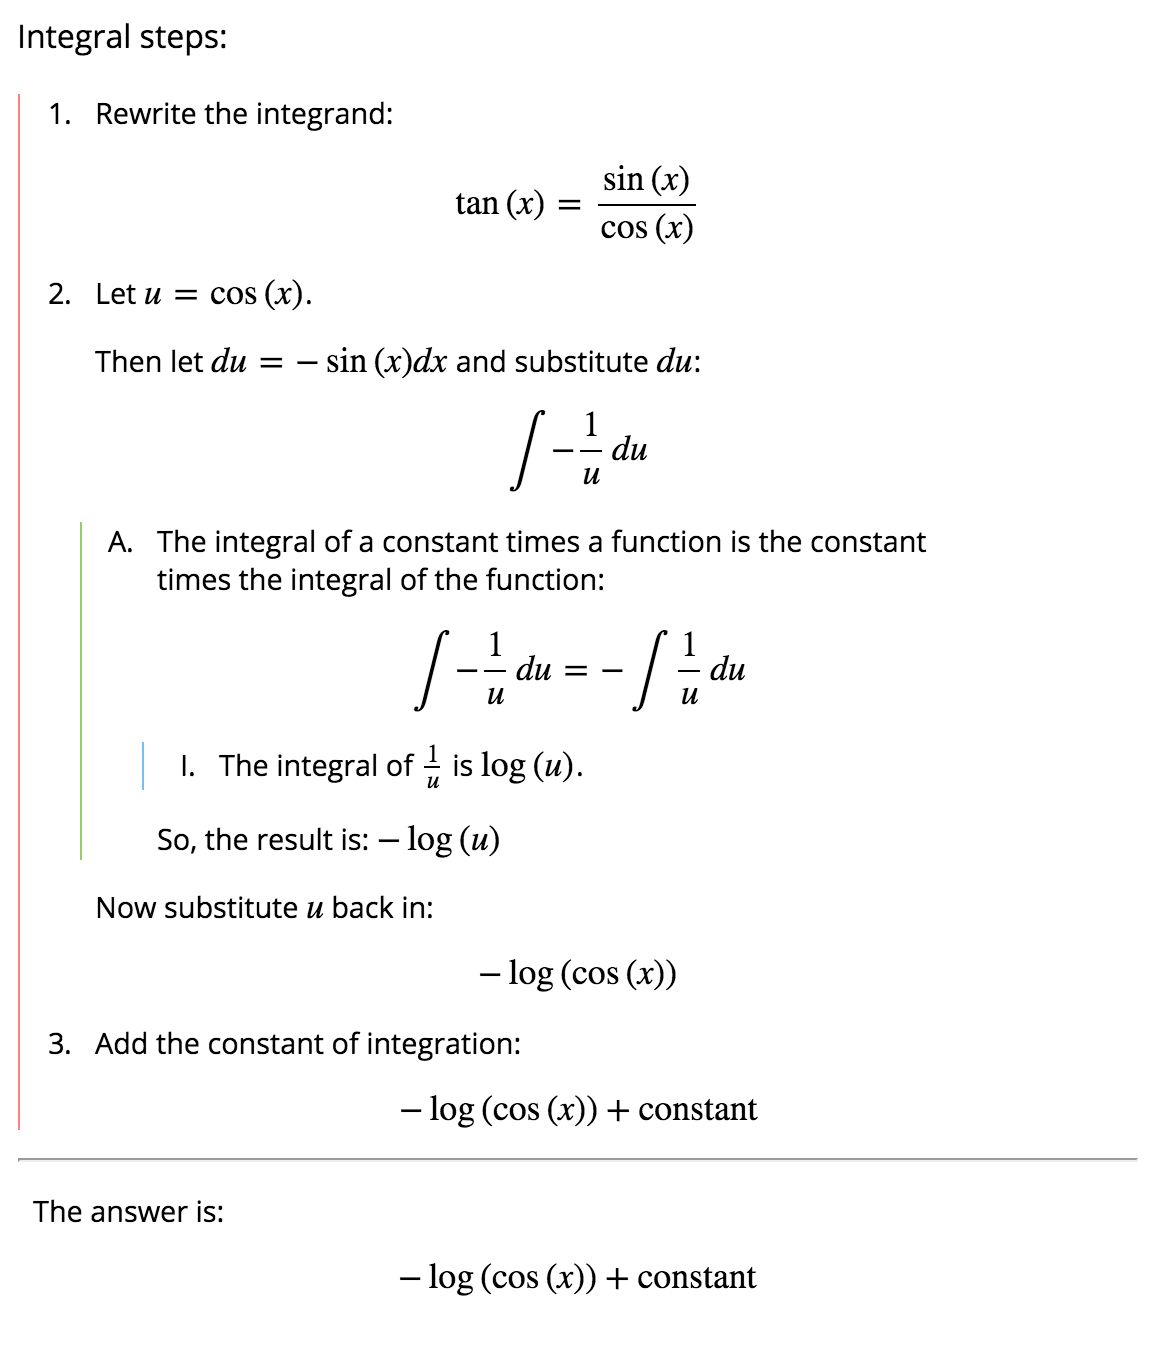
\includegraphics[width=0.7\textwidth]{supp-fig2-integral_steps.png}
    \captionof{figure}{\href{http://www.sympygamma.com/input/?i=integrate+tan\%28x\%29}{Integral steps of $\tan (x)$}.}\label{fig:integralsteps}
    \par
  }
\item
  SymPy Gamma displays the factor tree diagrams for different numbers.
\item
  SymPy Gamma saves user search queries.
\end{itemize}
Every input query from the user on SymPy Gamma is first parsed by its
own parser capable of handling several different forms of function names
which SymPy as a library does not support. For instance, SymPy Gamma
supports queries like \texttt{sin\ x}, whereas SymPy will only recognise
\verb|sin(x)|.

This parser converts the input query to the equivalent SymPy readable code,
which is then processed by SymPy, and the result is finally printed with the
built-in MathJax~\cite{cervone2012mathjax} output and rendered by the SymPy
Gamma web application.


\section{Comparison with Mathematica}
\label{suppsec:comp-mma}

Wolfram Mathematica is a popular proprietary CAS.\@
It features highly advanced algorithms.
Mathematica has a core implemented in C++~\cite{Wolfram2016}
which interprets its own programming language (know as Wolfram language).

% M-expressions

Analogously to Lisp's S-expressions,
Mathematica uses its own style of M-expressions,
which are arrays of either atoms or other M-expression.
The first element of the expression identifies the type of the expression
and is indexed by zero, whereas the first argument is indexed by one.
Notice that SymPy expression arguments are stored in a Python tuple
(that is, an immutable array),
while the expression type is identified by the type of the object storing the
expression.

% Attributes

Mathematica can associate attributes to its atoms.
Attributes may define mathematical properties and behavior of the nodes
associated to the atom.
In SymPy, the usage of static class fields is roughly similar to Mathematica's
attributes, though other programming patterns may also be used the achieve an
equivalent behavior, such as class inheritance.

% Expression mutability

Unlike SymPy, Mathematica's expressions are mutable,
that is one can change parts of the expression tree without the need of
creating a new object.
The reactivity of Mathematica allows for a lazy updating of any references
to that data structure.

% * comparison with Mathematica: commutativity, associative expressions, one-identity. Advantage of SymPy: multiplicative commutativity defined on symbols.
% Products and commutativity

Products in Mathematica are determined by some builtin node types,
such as \texttt{Times}, \texttt{Dot}, and others.
\texttt{Times} is overloaded by the * operator,
and is always meant to represent a commutative operator.
The other notable product is \texttt{Dot}, overloaded by the \texttt{.} operator.
This product represents matrix multiplication,
it is not commutative.
SymPy uses the same node for both scalar and matrix multiplication,
the only exception being with abstract matrix symbols.
Unlike Mathematica, SymPy determines commutativity with respect to
multiplication from the factor's expression type.
Mathematica puts the \texttt{Orderless} attribute on the expression
type.

% Associative expressions.

Regarding associative expressions,
SymPy handles associativity by making associative expressions inherit the
class \texttt{AssocOp},
while Mathematica specifies the \texttt{Flat}\cite{WolframRefFlat} attribute on the expression type.

% One identity


% Pattern matching

Mathematica relies heavily on pattern matching:
even the so-called equivalent of function declaration is in reality
the definition of a pattern matching generating an expression tree transformation
on input expressions.
%
Mathematica's pattern matching is sensitive to associative\cite{WolframRefFlat}, commutative\cite{WolframRefOrderless},
and one-identity\cite{WolframRefOneIdentity} properties of its expression tree nodes\cite{WolframRefFlatAndOrderlessFunctions}.
%
SymPy has various ways to perform pattern matching.
All of them play a lesser role in the CAS than in Mathematica
and are basically available as a tool to rewrite expressions.
The differential equation solver in SymPy somewhat relies on pattern matching to
identify the kind of differential equation, but it is envisaged to replace
that strategy with analysis of Lie symmetries in the future.
Mathematica's real advantage is the ability to add new overloading to the
expression builder at runtime, or for specific subnodes.
Consider for example
\begin{verbatim}
In[1]:= Unprotect[Plus]

Out[1]= {Plus}

In[2]:= Sin[x_]^2 + Cos[y_]^2 := 1

In[3]:= x + Sin[t]^2 + y + Cos[t]^2

Out[3]= 1 + x + y
\end{verbatim}
This expression in Mathematica defines a substitution rule that overloads
the functionality of the \texttt{Plus} node (the node for additions in Mathematica).
The trailing underscore after a symbol means that it is to be considered a
wildcard.
This example may not be practical, one may wish to keep this identity
unevaluated, nevertheless it clearly illustrates the potentiality to define
one's own immediate transformation rules.
In SymPy the operations constructing the addition node in the expression tree
are Python class constructors,
and cannot be modified at runtime.\footnote{In reality, Python supports monkey patching,
nonetheless it is a discouraged programming pattern.}
The way SymPy deals with extending the missing runtime overloadability functionality
is by subclassing the node types.
Subclasses may overload the class constructor to yield the proper
extended functionality.


%% TODO list:
% * comparison with Mathematica: MatrixExp, product not always commutative, type inheritance (polymorphism) and advantage in unifying the product symbol * for symbols and matrices, pattern matching vs. single dispatch.

% Type inheritance and polymorphism

Unlike SymPy, Mathematica does not support type inheritance or polymorphism~\cite{Fateman1992}.
% cite examples of class inheritance in SymPy:
%
SymPy relies heavily on class inheritance, but for the most part,
class inheritance is used to make sure that SymPy objects inherit the proper
methods and implement the basic hashing system.
Associativity of expressions can be achieved by inheriting the class \texttt{AssocOp},
which may appear a more cumbersome operation than Mathematica's attribute setting.
%There are also cases where inheritance is used to extend the mathematical meaning of an expression.

% Matrices

Matrices in SymPy are types on their own.
In Mathematica, nested lists are interpreted as matrices whenever the sublists
have the same length.
The main difference to SymPy is that ordinary operators and functions
do not get generalized the same way as used in traditional mathematics.
Using the standard multiplication in Mathematica performs an elementwise
product, this is compatible with Mathematica's convention of commutativity of
\texttt{Times} nodes.
Matrix product is expressed by the \textit{dot} operator,
or the \texttt{Dot} node.
The same is true for the other operators, and even functions,
most notably calling the exponential function \texttt{Exp} on a matrix
returns an elementwise exponentiation of its elements.
The real matrix exponentiationl is available through the \texttt{MatrixExp}
function.

% * comparison with Mathematica: avoid misspelling variables through forced declaration (check that you can't do it in Mathematica).
% * evaluate=False vs HoldForm

Unevaluated expressions can be achieved in various ways,
most commonly with the \texttt{HoldForm} or \texttt{Hold} nodes,
that block the evaluation of subnodes by the parser.
Note that such a node cannot be expressed in Python, because of greedy evaluation.
Whenever needed in SymPy, it is necessary to add the parameter \texttt{evaluate=False}
to all subnodes, or put the input expression in a string.

% * comparison with Mathematica: == is structural equality, not

The operator == returns a boolean whenever it is able to immediately evaluate
the truthness of the equality, otherwise it returns an \texttt{Equal} expression.
In SymPy == means structural equality and is always guaranteed to return a
boolean expression.
To express an equality in SymPy it is necessary to explicitly construct the
\texttt{Equality} class.

% * comparison with Mathematica: polynomial module.
% * comparison with Mathematica: space is product, ** vs ^

SymPy, in accordance with Python and unlike the usual programming convention,
uses ** to express the power operator, while Mathematica uses the more
common \verb|^|.

% * comparison with Mathematica: ( ) is Sequence, functions are generally uppercase.
% * comparsion with Mathematica: table of comparison?
% * comparison with Mathematica: Wolfram language has loads of operator overloading, functional paradigm.


\bibliography{paper}

\end{document}
